\chapter{Etude Comparative et Choix du Modèle}
\section{Introduction}
Tout d'abord, nous allons présenter dans ce chapitre l'architecture de notre solution avec tous les composants nécessaires, puis nous allons reprendre les critères de comparaison présentés dans le cadre méthodologique. Pour évaluer les modèles CNN existants dans la bibliothèque Keras. 

Ensuite, nous allons trier ces modèles et tirer les quatre meilleurs modèles par rapport aux critères définis précédemment. Ces modèles seront implémentés dans un cas réel afin de comparer leurs performances en pratique.  

A la fin de ce chapitre, nous allons sélectionner le modèle le plus approprié pour notre application. 

\section{Architecture de la solution}
L'approche consiste à créer une application de vision artificielle capable d'utiliser une caméra de détection pour distinguer les nouilles conformes des nouilles non conformes. La caméra capture des images des nouilles pendant leur déplacement sur la ligne de production. Ces images sont capturées en temps réel à l'aide d'une photocellule qui détecte l'arrivée des nouilles et transmet des impulsions électriques à la caméra pour capturer la zone de détection. 

Les images sont envoyées à la base de données du logiciel pour être traitées en temps réel. Ce logiciel est implémenté dans un TPU qui est le cerveau de l'ensemble du système. Ce TPU dispose d'un modèle d'apprentissage profond qui peut traiter ces images et distinguer les nouilles conformes et non-conformes en fonction des caractéristiques qui ont été entraînées auparavant. Nous détaillerons la phase d'entraînement du modèle dans la suite de ce chapitre. Le modèle comprend les caractéristiques de la nouille et cela signifie que s'il y a un changement dans les caractéristiques de la nouille, il trouvera s'il s'agit d'un changement normal, donc la nouille est toujours conforme, ou d'un changement anormal, donc la nouille est non conforme. 
\newpage
Suite à la réponse du modèle, autrement dit l'inférence, le TPU délivre un signal au vérin à l'aide de broches d'entrée/sortie. Si la nouille est conforme, le vérin réagit en fonction de l'inférence et la laisse passer. Si elle n'est pas conforme, elle sera poussée hors du convoyeur et placée dans un sac spécial pour les nouilles non conformes .la figure ci-dessous représente un schéma explicatif sur la solution complète : 

\begin{figure}[h]
    \centering
    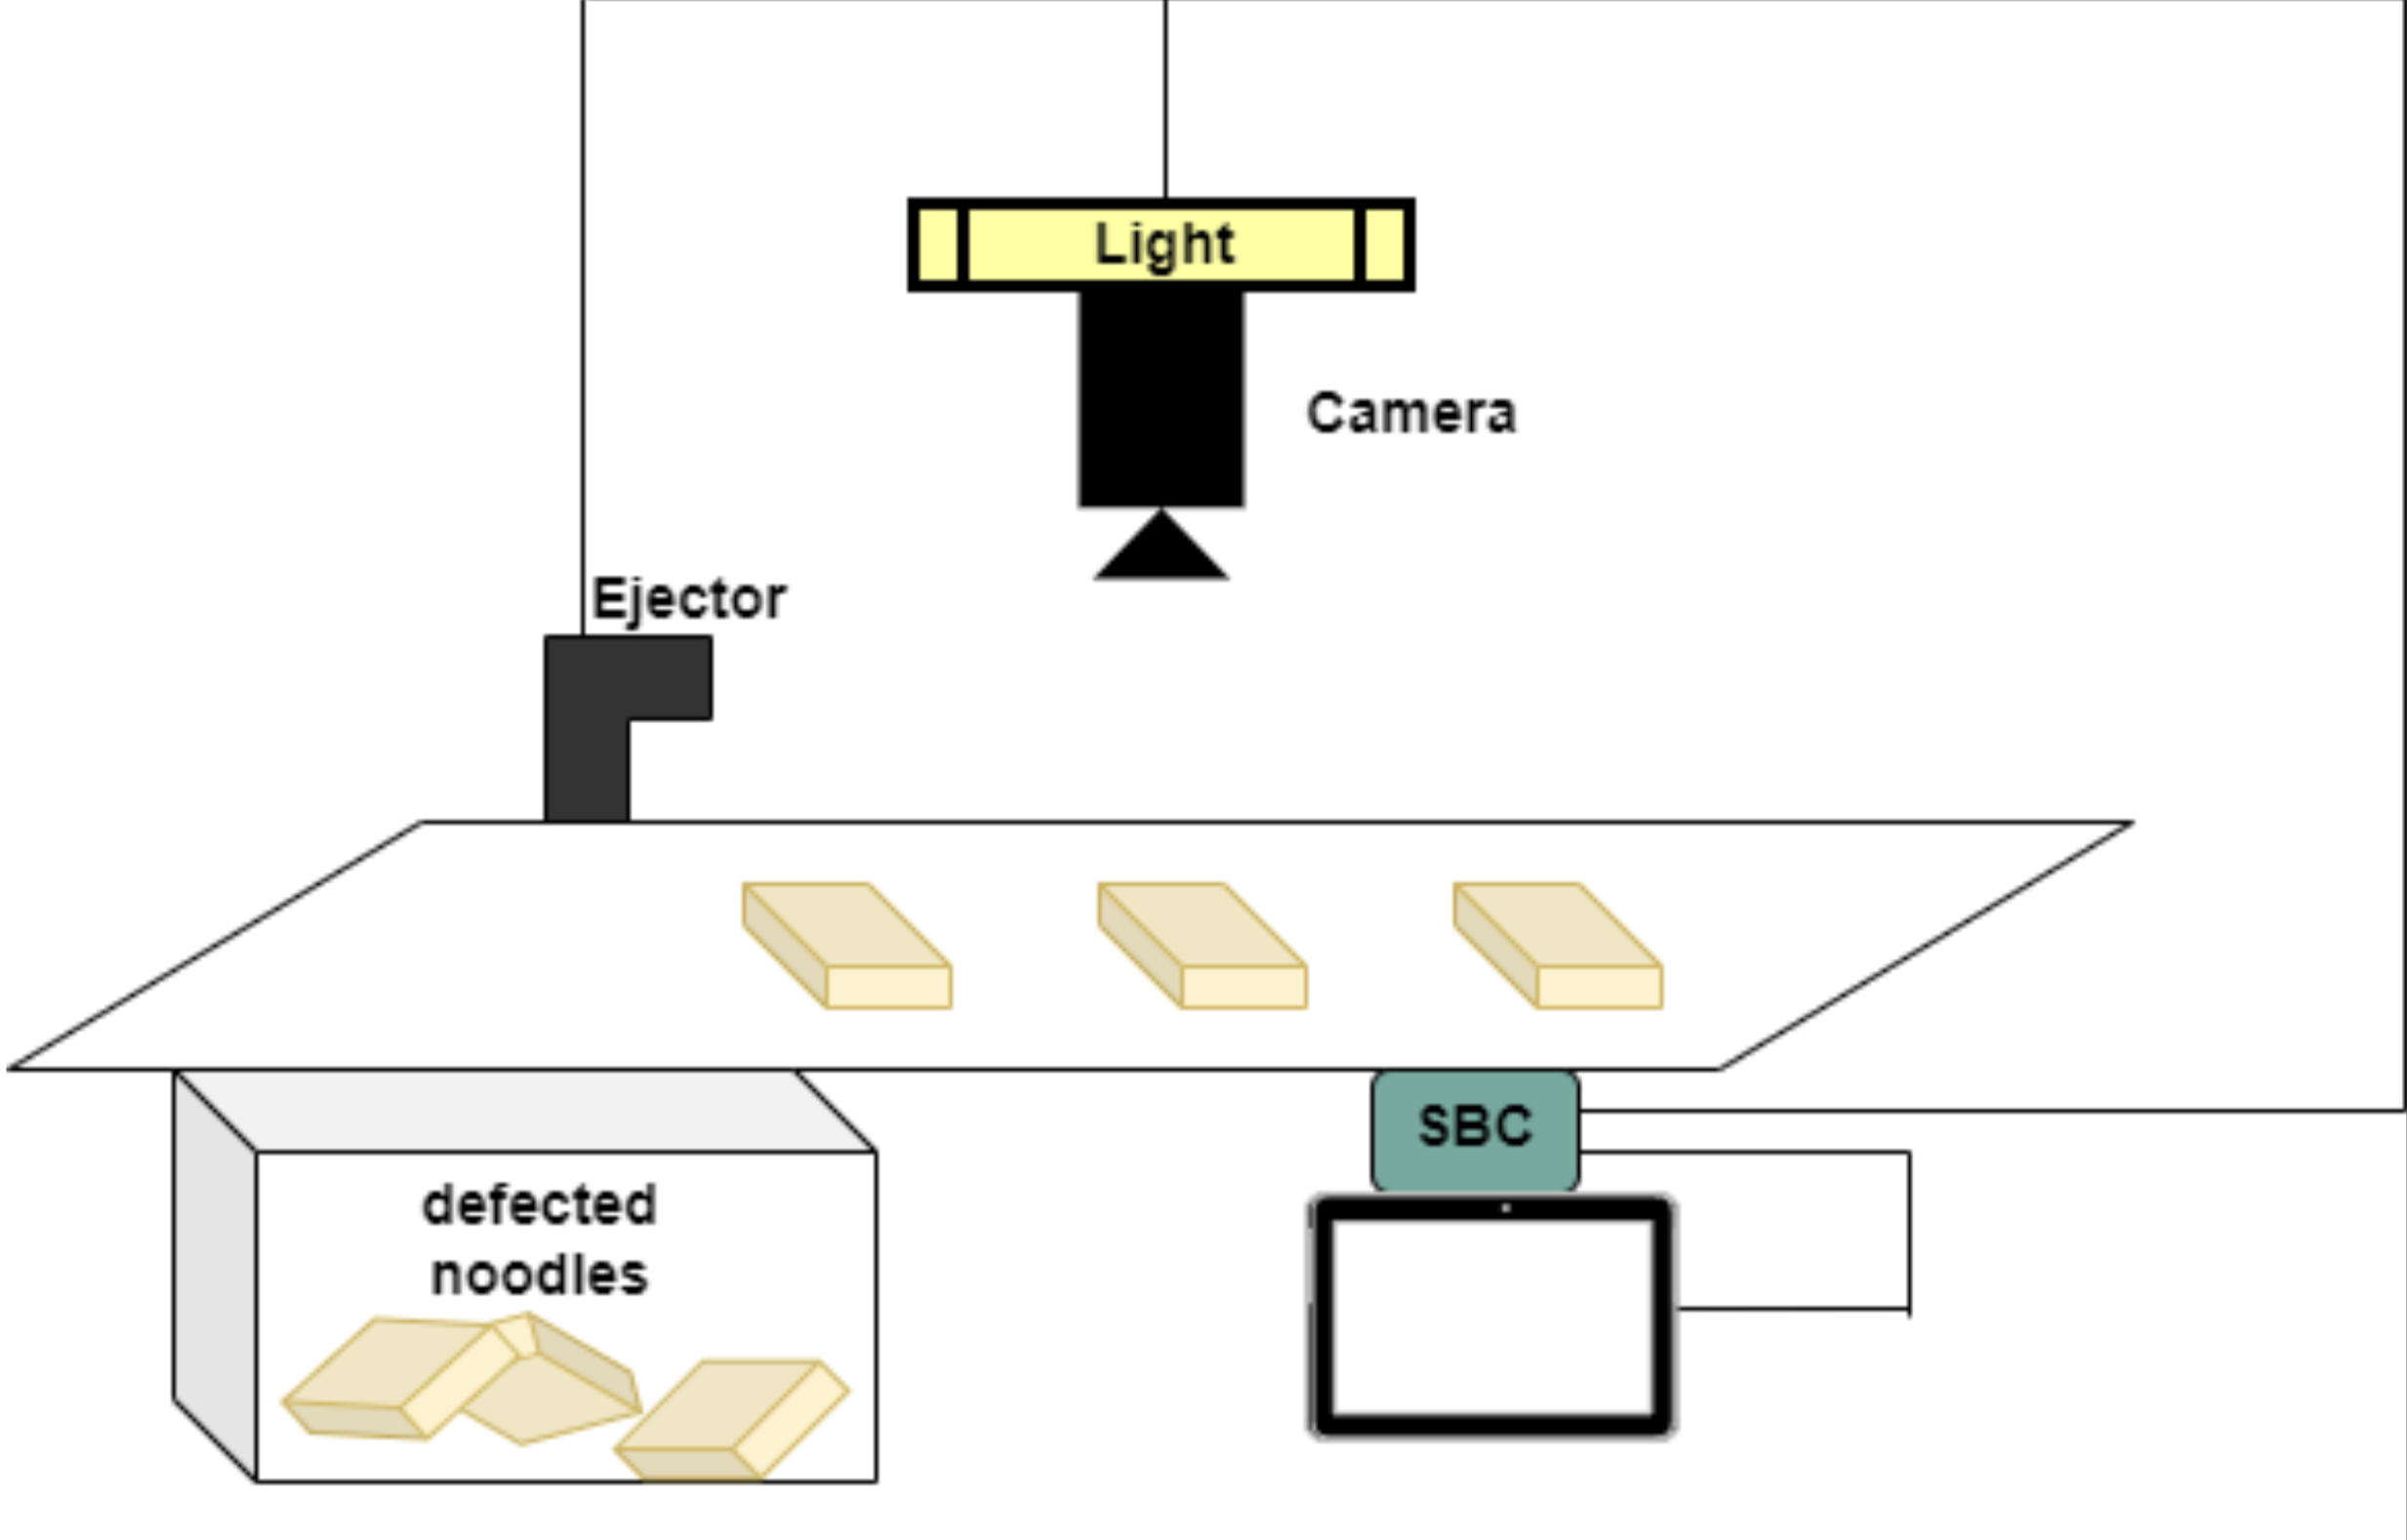
\includegraphics[width=10cm]{assets/PartTwo/Chapterone/ShemaExplicatif.png}
    \caption{Schema explicatiof}
    \label{SchemaArchitecture}
    \end{figure}

Pour faciliter le travail, le logiciel devra être commandé par une interface utilisateur graphique (GUI) moderne et simple, l'interface est représentée sur un écran tactile pour permettre à l'opérateur de contrôler le système, de le configurer, d'extraire les résultats et de voir les statistiques en temps réel .la figure suivante représente GUI de notre système :
GuiInterface 
\begin{figure}[h]
    \centering
    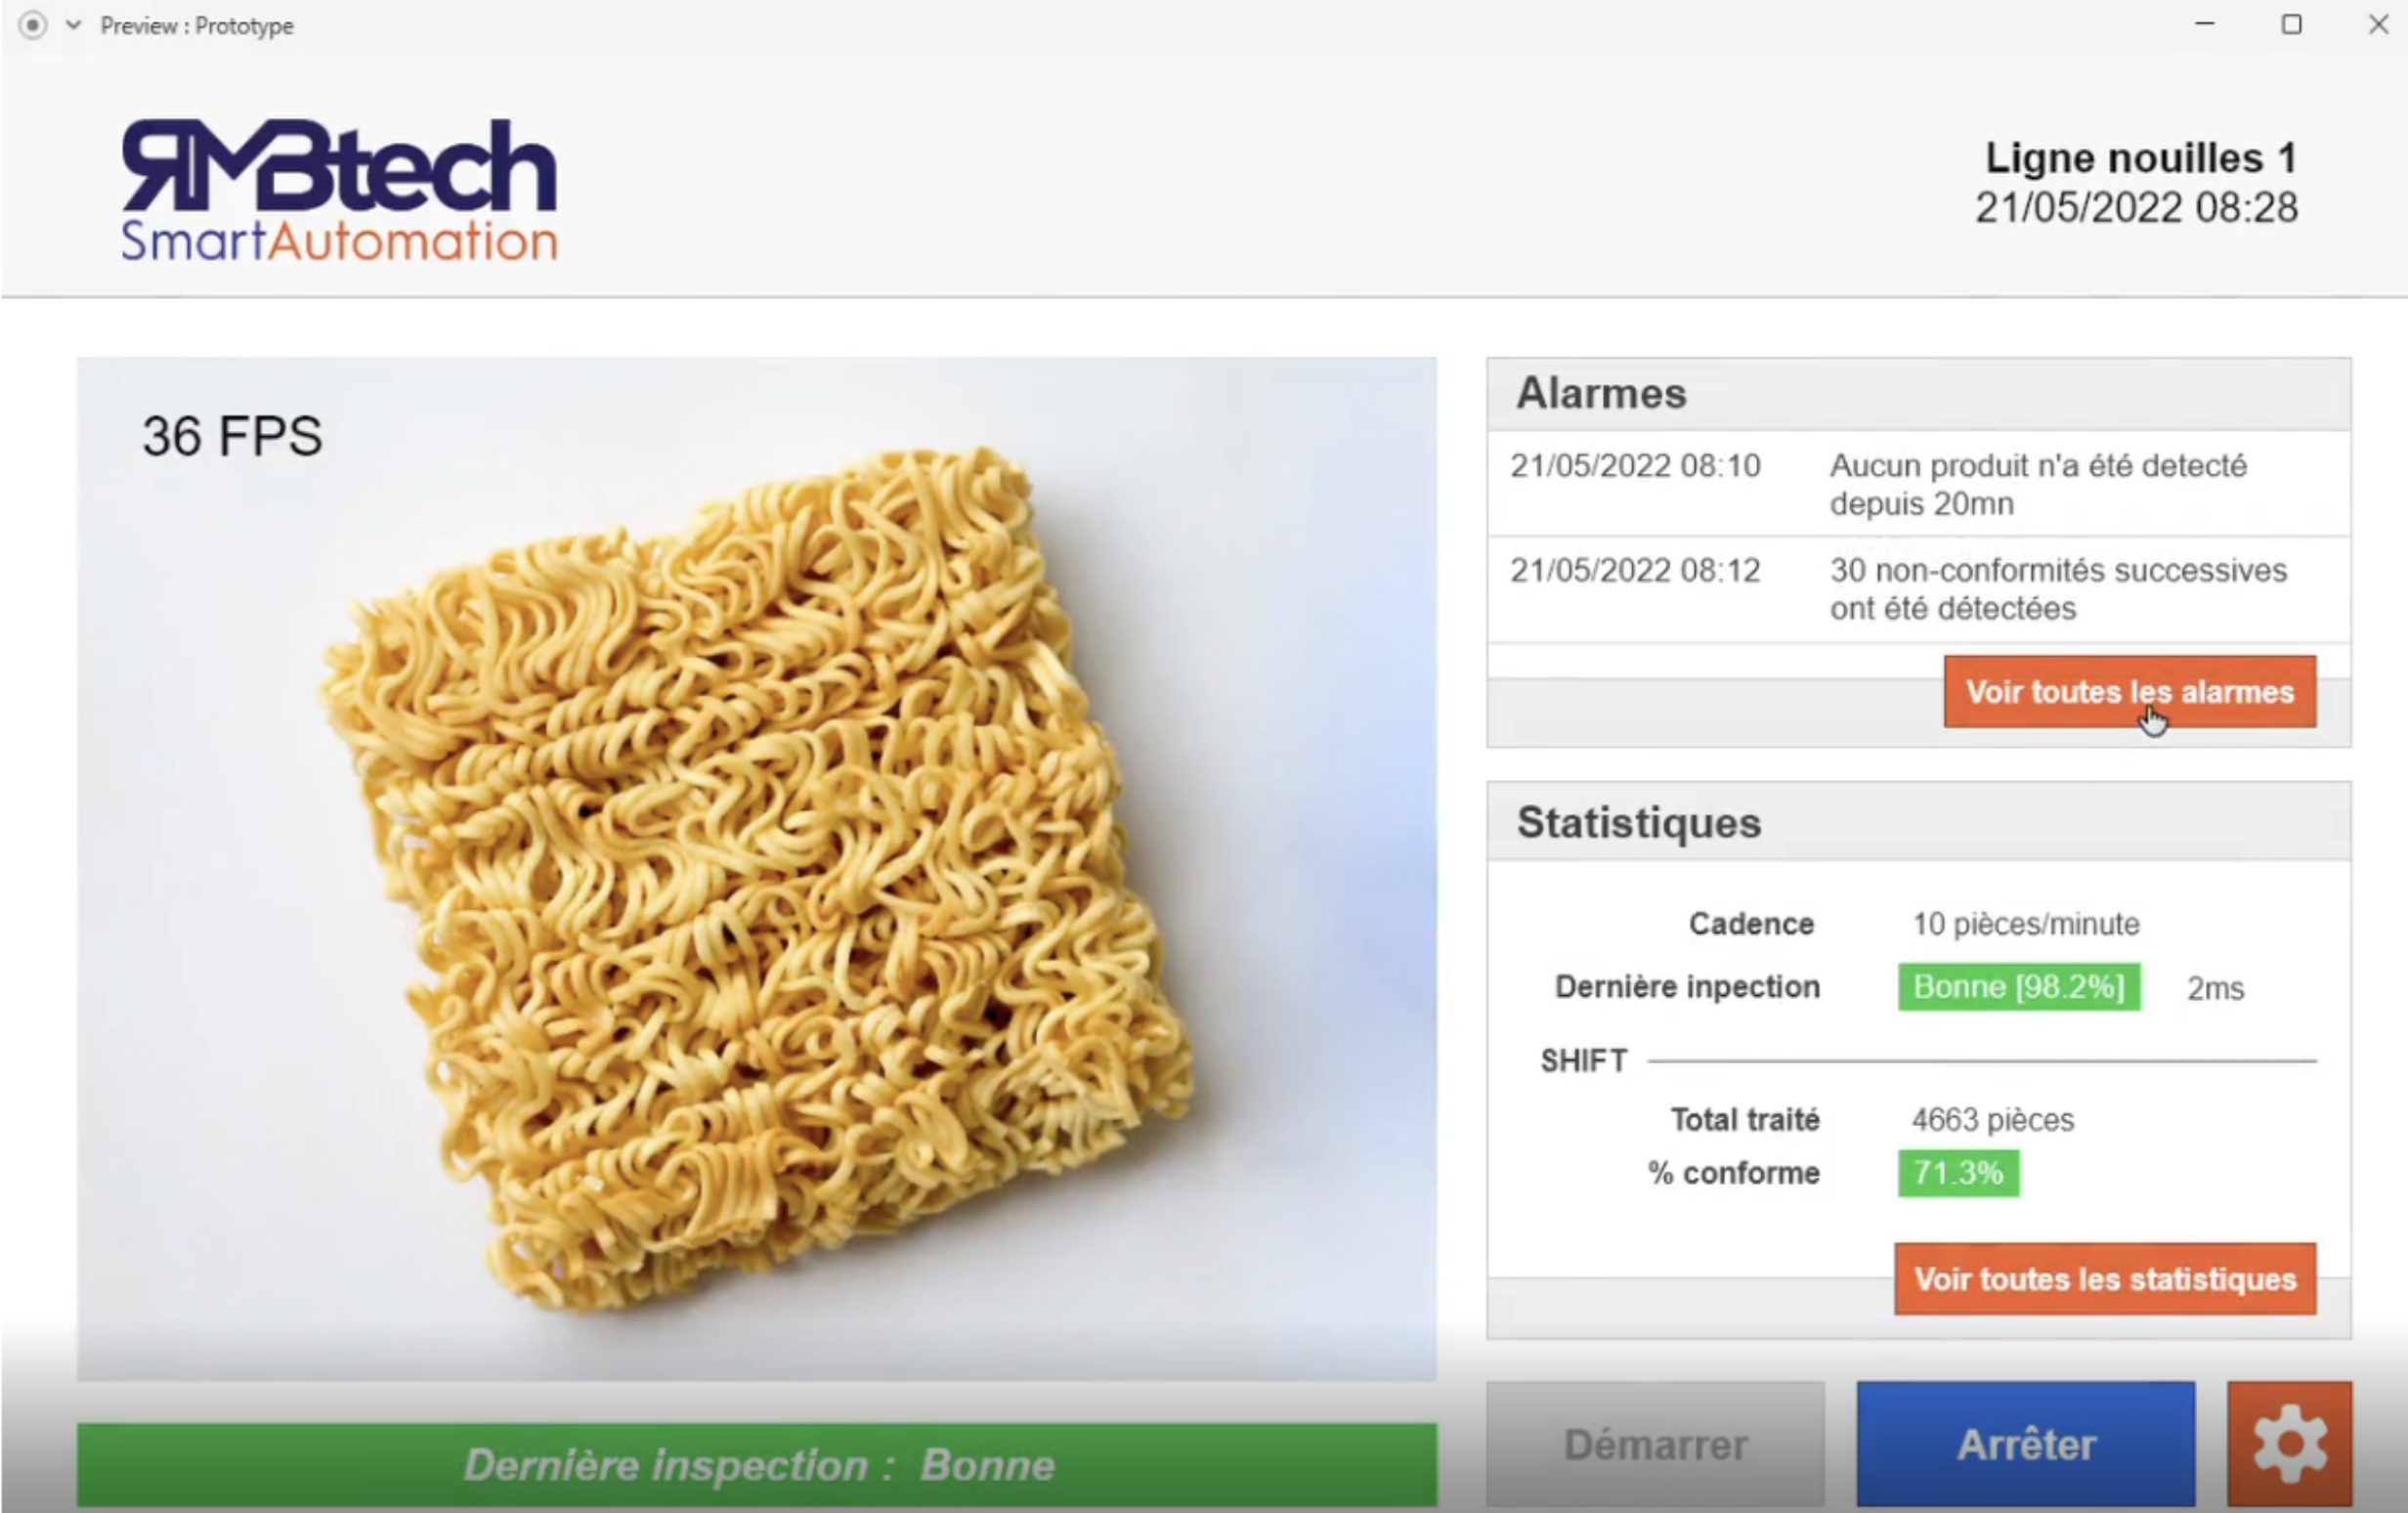
\includegraphics[width=12cm]{assets/PartTwo/ChapterTwo/GuiInterface.png}
    \caption{GUI}
    \label{GUI}
    \end{figure}

\newpage
\section{Configuration Hardware et Software}
Dans ce point, nous allons décrire les choix techniques de l'ensemble de la partie matérielle (Hardware) et partie logiciel (Software). 
\subsection{Choix de la caméra : }
Nous avons choisi une caméra à zone de balayage car elle nous permet de recevoir rapidement une image de la zone des nouilles, et dans le cas d'un contrôle de non-conformité en temps réel, la vitesse du système est un facteur critique. Pour des raisons de rapidité également nous avons fixé la résolution à 800*600 et cela augmentera les FPS c'est-à-dire augmentera la vitesse de capture de la caméra. Lorsque la nouille traverse le champ de la photocellule l'image est capturée. Dont le champ de détection de la photocellule est de 6 cm. 
\subsection{Choix d'éclairage : }
Nous avons utilisé un éclairage frontal avec une ampoule LED circulaire pour diriger la lumière vers les nouilles et éliminer les régions secondaires pour garder un focus et un contraste total sur la zone de détection de la nouille. 
\subsection{Choix du TPU : }
Nous avons utilisé le TPU Asus Tinker Edge T qui est utile pour les applications industrielles car il a une capacité de traitement élevée. Tous ces composants sont rassemblés dans un support métallique qui est installé sur une bande transporteuse et sont alimentés par une source de tension de 24V.  

\section{Préparation des données }
Notre recherche vise à catégoriser l'image des nouilles. L'ensemble de données d'entraînement et de test ont été créés à partir de l'ensemble de données original. Un ensemble de données contenant 4000 images a été utilisé dans ce travail pour l'entrainement, devisé en deux classe GOOD et DEFECT chaque classe contient 2000 images pour la validation on a pris 1000 images. Les images ont été choisies au hasard.  

L'image originale de l'appareil photo a une taille de 800 x 600 pixels. Le centre de l'image est l'endroit où se trouvent les nouilles. Les images ont été réduites à 224 x 224 pixels afin de réduire la complexité du traitement et d'être compatibles avec l'entrée du modèle. 

\newpage
La figue \ref{GoodDefectNoodles} montre un échantillon des données avec ces deux classes GOOD et DEFECT 
\begin{figure}[h]
    \centering
    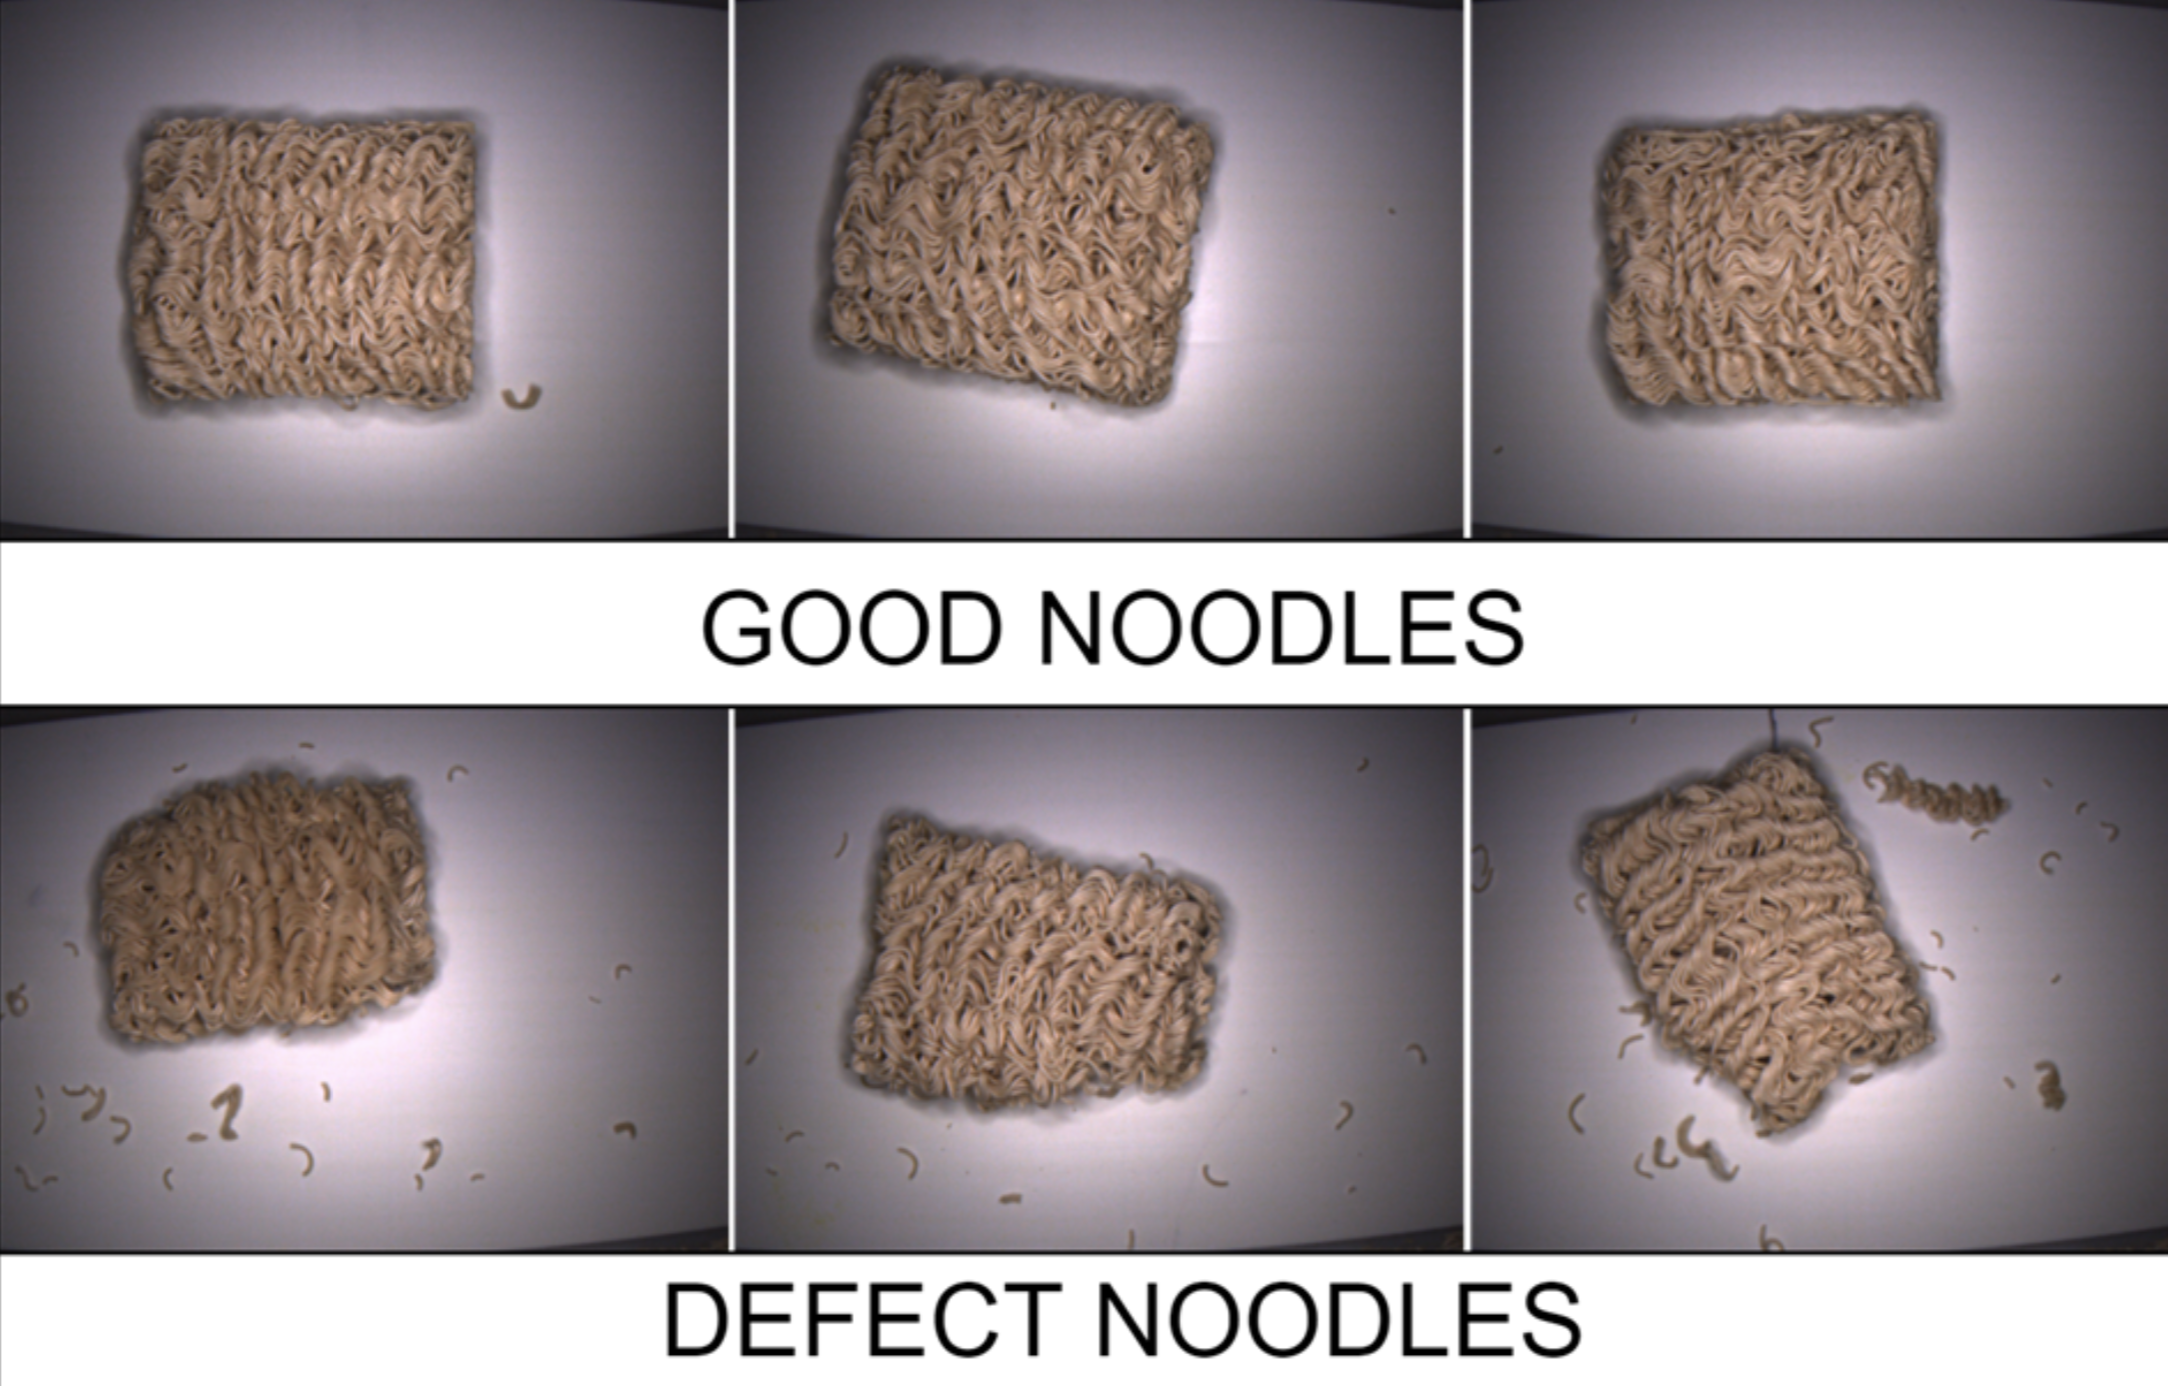
\includegraphics[width=14cm]{assets/PartTwo/ChapterTwo/GoodDefectNoodles.png}
    \caption{GoodDefectNoodles}
    \label{GoodDefectNoodles}
    \end{figure}

\section{Implémentation des modèles}
Notre travail consiste à utiliser des modèles pré-entraînés de Keras et nous allons les réentraîner avec nos données. Cette technique est appelée transfert learning, et nous l'avons abordée plus en détail dans le chapitre deux de la première partie.  
Une première sélection théorique a été faite manuellement à travers une comparaison des trois critères sur tous les modèles de Keras.  

Cette comparaison théorique a été faite à l'aide d'une matrice de décision où nous avons donné à chaque critère une note sur 10, nous n'avons pas utilisé de pondération car les trois critères ont la même importance. Le Tableau ci-dessous montre le tableau de comparaison des modèles. 
\newpage
\begin{figure}[h]
    \centering
    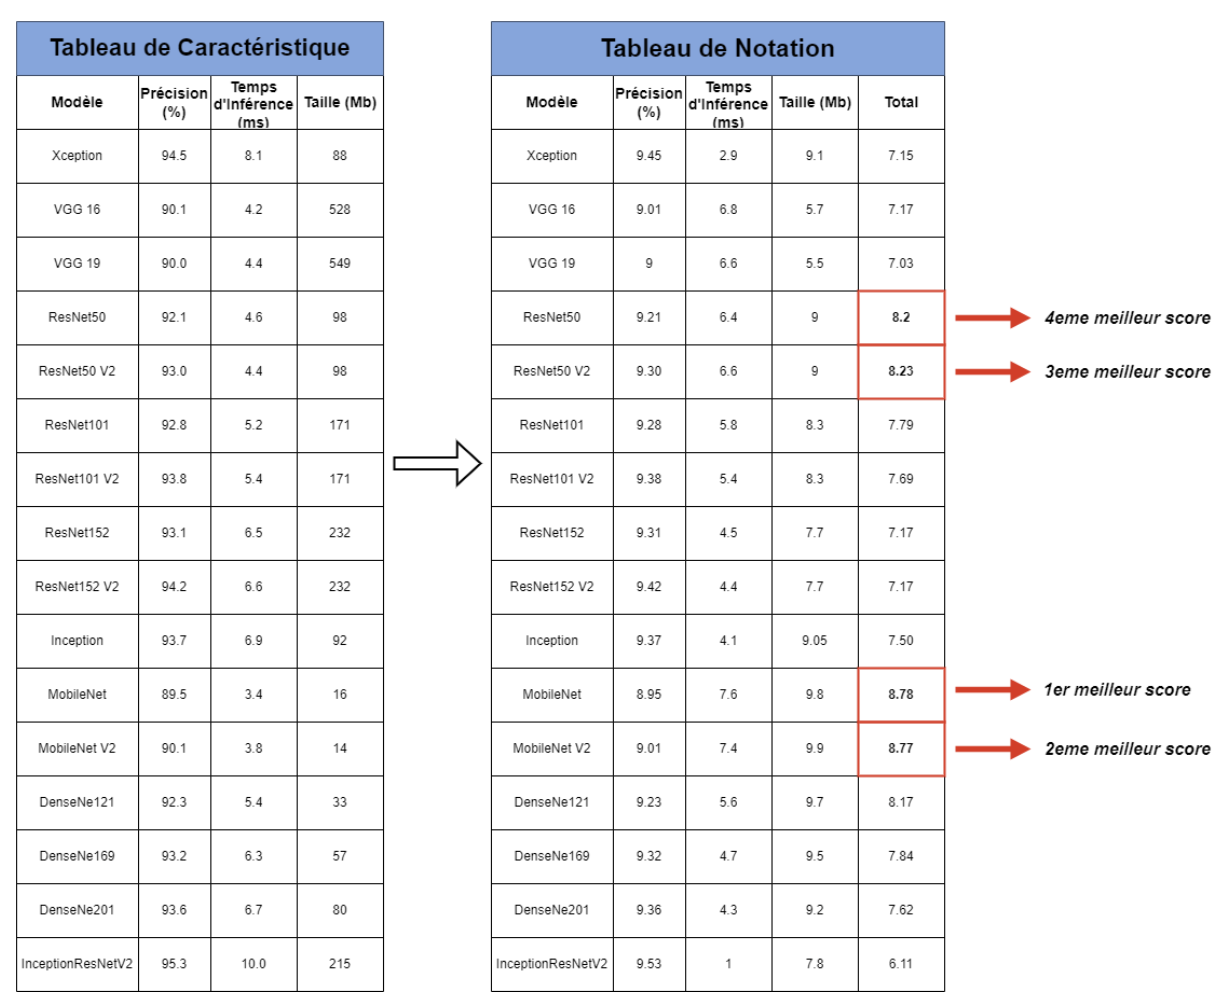
\includegraphics[width=14cm]{assets/PartTwo/ChapterTwo/ComparaisonModeles.png}
    \caption{ComparaisonModeles}
    \label{ComparaisonModeles}
    \end{figure}

    D'après la figure, nous pouvons voir que quatre modèles ont été sélectionnés et qu'ils sont les suivants : MobileNet, MobileNet V2, ResNet50, ResNet50 V2.

    Les architectures de ces modèles ont été détaillé dans le chapitre deux de la première partie. 

\section{Evaluation des modèles}
Dans cette section, nous présenterons une évaluation des caractéristiques utilisées pour comparer les performances des quatre modèles, ainsi que les résultats produits et une discussion des résultats des modèles décrits. 

Tous les modèles de cette section ont été créés avec des hyperparamètres distincts. Ces derniers ont été choisis après de multiples itérations, et pour chaque modèle, nous avons pris les hyperparamètres qui ont donné les meilleurs résultats. 


Les détails des résultats pour chaque modèle est présenté ci-dessous : 
\newpage
\subsection{MobileNet V1 }
Concernant le MobileNet, nous avons utilisé les hyperparamètres détaillés dans le tableau suivant : 

    \begin{table}[h]
        \begin{center}
            \begin{tabular}{|l|l|l|l|}
                \hline
                Forme de l'entrée & Taille du lot & Epoques & Taux d'apprentissage \\ \hline
                (224, 224)        & 32            & 500     & 5e-5                 \\ \hline
                \end{tabular}
        \end{center}
        
        \end{table}
        Le modèle atteint une précision de 99.25\% à l'entraînement et 98.21\% en teste, le taux d’erreur pour l'entraînement et le teste est respectivement 1.17\%, 8.37\%. Ce qui montre un bon résultat vu que l’erreur ne dépasse pas 10\%. Les résultats de l'entraînement et des tests de ce modèle sont présentés dans la Figure \ref{MobileNetV1Result}. 
 \begin{figure}[h]
\centering
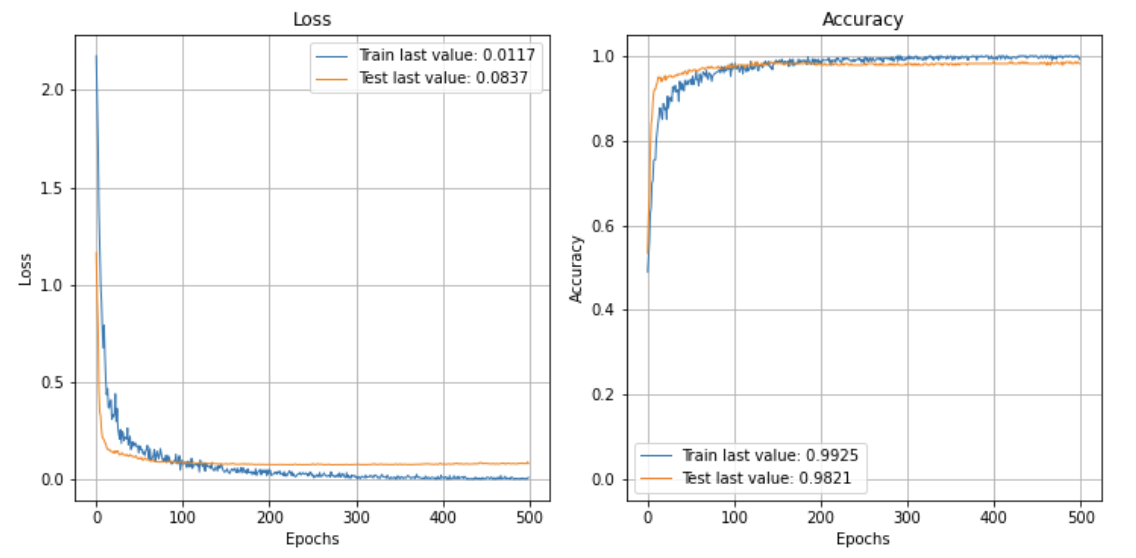
\includegraphics[width=13cm]{assets/PartTwo/ChapterTwo/MobileNetV1Result.png}
\caption{MobileNetV1Result}
\label{MobileNetV1Result}
\end{figure}

Lors de l'implémentation du modèle, nous avons trouvé les résultats suivants : la taille et le temps d'inférence pratique sont respectivement de 9,4 Mo et 3,07 ms, en ce qui concerne la précision pratique (validation), nous avons trouvé la matrice de confusion présentée dans la Figure \ref{MOBILENETV1TFTV} qui donne une précision de 96,35\%. 

\begin{figure}[h]
    \centering
    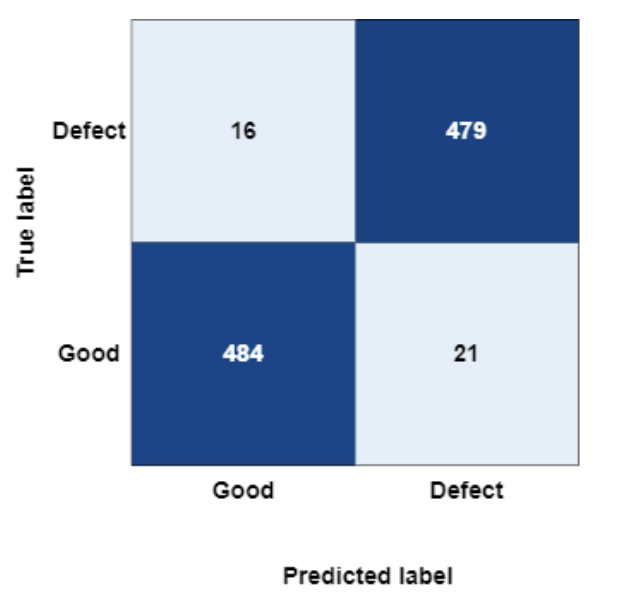
\includegraphics[width=5cm]{assets/PartTwo/ChapterTwo/MOBILENETV1TFTV.png}
    \caption{MOBILENETV1TFTV}
    \label{MOBILENETV1TFTV}
    \end{figure}
\newpage
\subsection{MobileNet V2}
Le MobileNet V2 a été entraîné avec les mêmes hyperparamètres sauf qu’on a changé le taux d’apprentissage à 1e-7. Le Tableau suivant montre les hyperparamètres d'entraînement du MobileNet V2. 
\begin{table}[h]
    \begin{center}
        \begin{tabular}{|l|l|l|l|}
            \hline
            Forme de l'entrée & Taille du lot & Epoques & Taux d'apprentissage \\ \hline
            (224, 224)        & 32            & 500     & 1e-7                 \\ \hline
            \end{tabular}
    \end{center}
    
    \end{table}
    Ce modèle a également obtenu de bons résultats en termes de précision et d'erreur. Il a atteint une précision à l'entraînement et au test de 99,75\% et 97,85\%, respectivement, l'erreur n'a pas dépassé 10\% et s'est située entre 1,21\% à l'entraînement et 7,73\% au test. La Figure \ref{MobileNetV2Result} montre les résultats d'entraînement et de test de ce modèle. 
    \begin{figure}[h]
        \centering
        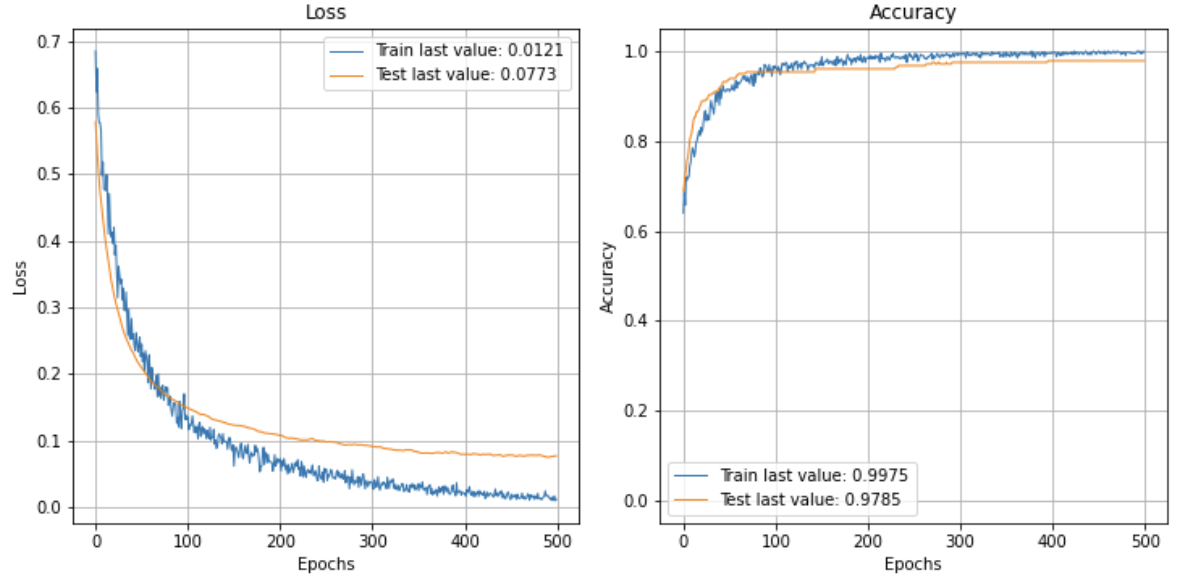
\includegraphics[width=13cm]{assets/PartTwo/ChapterTwo/MobileNetV2Result.png}
        \caption{MobileNetV2Result}
        \label{MobileNetV2Result}
        \end{figure}

La taille du modèle après implémentation est de 37,7 Mo, le temps d'inférence est de 3,9 ms et la précision de validation est de 95,9\% après le calcul de la matrice de confusion présentée à la figure \ref{MobileNetV2TFTN}.

\begin{figure}[h]
    \centering
    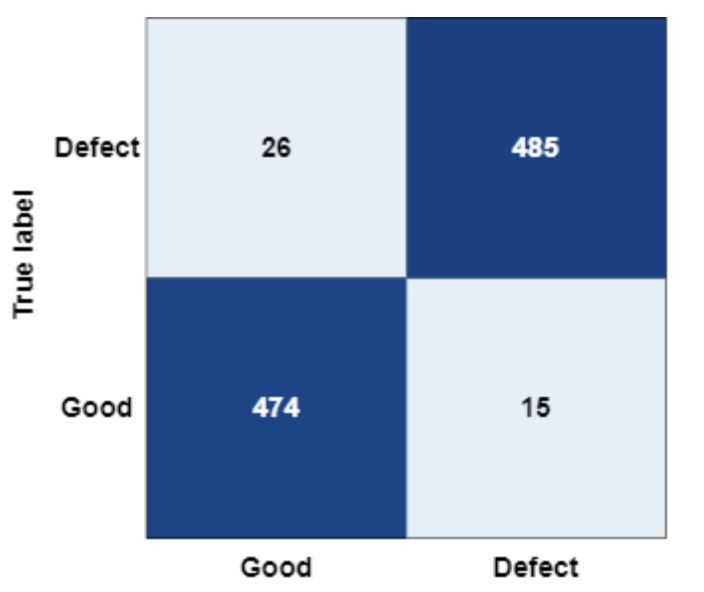
\includegraphics[width=6cm]{assets/PartTwo/ChapterTwo/MobileNetV2TFTN.png}
    \caption{MobileNetV2TFTN}
    \label{MobileNetV2TFTN}
    \end{figure}
\newpage
\subsection{ResNet50 V1 }
Pour ResNet50 V1, nous avons changé le taux d'apprentissage à 1e-5 et la taille du lot à 16. Ces hyperparamètres ont montré les meilleurs résultats pour les itérations de ResNet50 V1 et ont été représentés dans le tableau  suivant : 

\begin{table}[h]
    \begin{center}
        \begin{tabular}{|l|l|l|l|}
            \hline
            Forme de l'entrée & Taille du lot & Epoques & Taux d'apprentissage \\ \hline
            (224, 224)        & 16            & 500     & 1e-5                 \\ \hline
            \end{tabular}
    \end{center}
    \end{table}
    La précision de ce modèle était excellente, puisqu'elle était de 100\% pendant la formation et de 97,13\% pendant le test. Cependant, lorsque nous regardons l'erreur, nous observons que le modèle a plus de 14\% pour le test, ce qui indique un Overfitting donc le modèle n'est pas fiable en termes de précision. La Figure 2-6a montre les résultats de ResNet50 V1. 

    \begin{figure}[h]
        \centering
        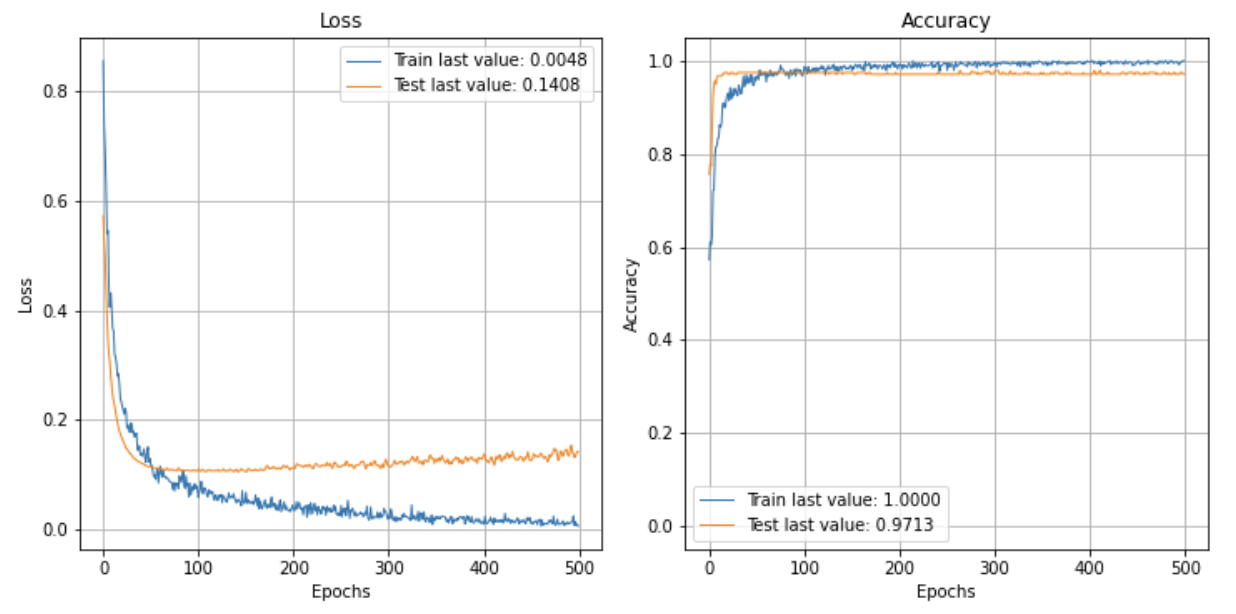
\includegraphics[width=13cm]{assets/PartTwo/ChapterTwo/ResNet50Results.png}
        \caption{ResNet50Results}
        \label{ResNet50Results}
        \end{figure}

Le modèle pratique a une taille de 103,2 Mo, avec un temps d'inférence de 5,1 ms. La précision pratique est de 88,1\%, et les propriétés de cette précision sont illustrées à la figure 2-6b. 
\begin{figure}[h]
    \centering
    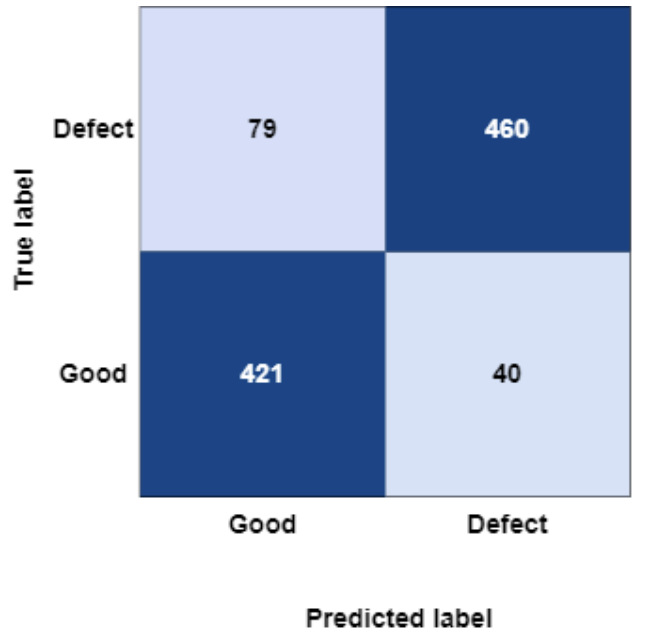
\includegraphics[width=5cm]{assets/PartTwo/ChapterTwo/ResNet50TFTN.png}
    \caption{ResNet50TFTN}
    \label{ResNet50TFTN}
    \end{figure}
\newpage

\subsection{ResNet50 V2 }
Enfin, pour ResNet50 V2, nous avons laissé la taille du lot à 32 et modifié le taux d'apprentissage à 2e-7. Le Tableau 2-5 suivant montre les hyperparamètres d'entraînement du ResNet50 V2. 
\begin{table}[h]
    \begin{center}
        \begin{tabular}{|l|l|l|l|}
            \hline
            Forme de l'entrée & Taille du lot & Epoques & Taux d'apprentissage \\ \hline
            (224, 224)        & 32            & 500     & 2e-7                  \\ \hline
            \end{tabular}
    \end{center}
    \end{table}
    Avec ces hyperparamètres, le modèle a atteint 99,5\% en entraînement et 98.21\% en test. Le modèle a atteint 1,43\% pendant l'entraînement et 6,34\% pendant les tests. La Figure \ref{ResNet50V2RESULT} montre les résultats d'entraînement et de test de ce modèle.
    \begin{figure}[h]
        \centering
        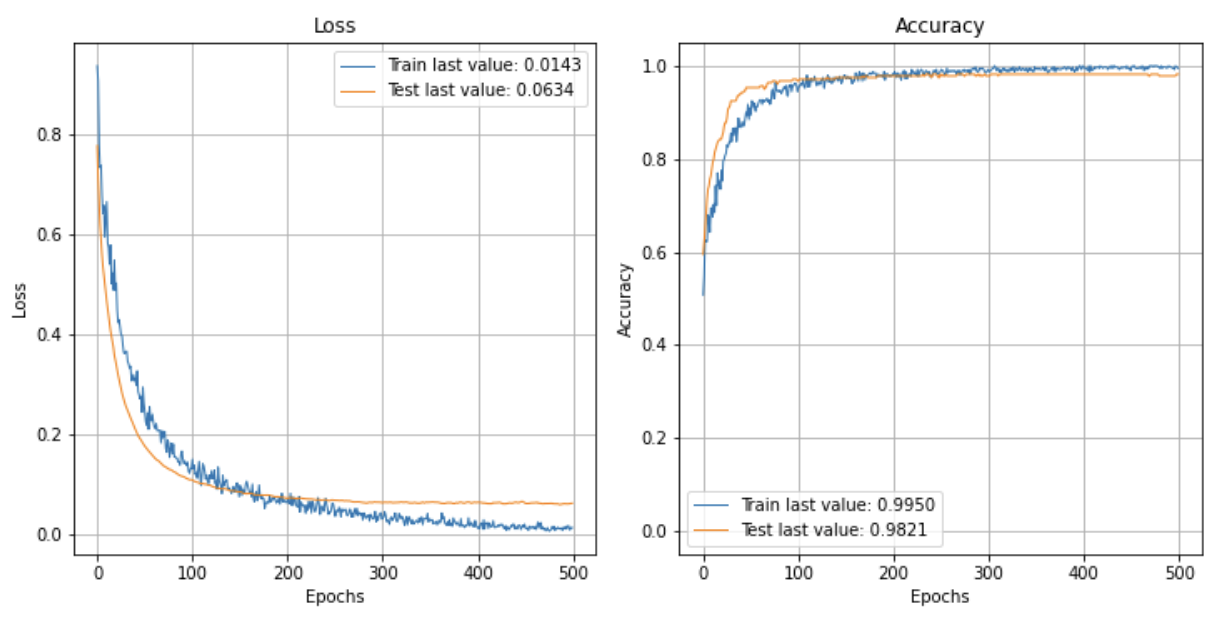
\includegraphics[width=13cm]{assets/PartTwo/ChapterTwo/ResNetV2RESULT.png}
        \caption{ResNetV2RESULT}
        \label{ResNet50V2RESULT}
        \end{figure} 
        La matrice de confusion présenté dans la Figure \ref{ResnetV2TFTD} a donné une précision pratique de 93,3\%. La taille de l'implémentation du modèle est de 322,8 Mo, et le temps d'inférence est de 9,3 ms. 

    \begin{figure}[h]
            \centering
            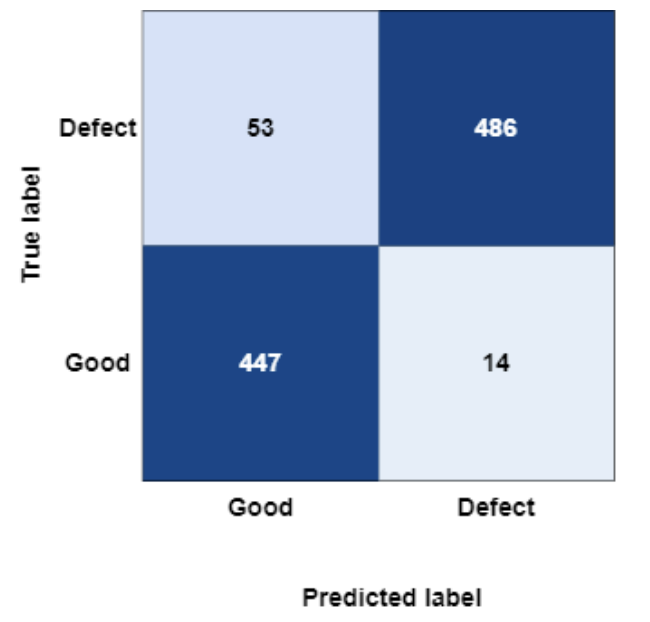
\includegraphics[width=5cm]{assets/PartTwo/ChapterTwo/ResnetV2TFTD.png}
            \caption{ResnetV2TFTD}
            \label{ResnetV2TFTD}
            \end{figure}
        \newpage
\section{Analyses et discussion des résultats}
Les résultats ci-dessus expliquent l'évaluation de chaque modèle. Comme une analyse à partir de ces résultats, nous pouvons effectuer une comparaison entre les quatre modèles en fonction des caractéristiques définies précédemment :la précision, le temps d'inférence, et la taille du modèle. 

Cette comparaison implique l'exécution d'une autre matrice de décision, similaire à celle présentée dans le tableau \ref{ComparaisonModeles}, afin d'évaluer les différences entre les caractéristique pratique de chaque modèle et de sélectionner le meilleur modèle à appliquer dans notre système. La figure suivante montre la comparaison entre les quatre modèles : 
\begin{figure}[h]
    \centering
    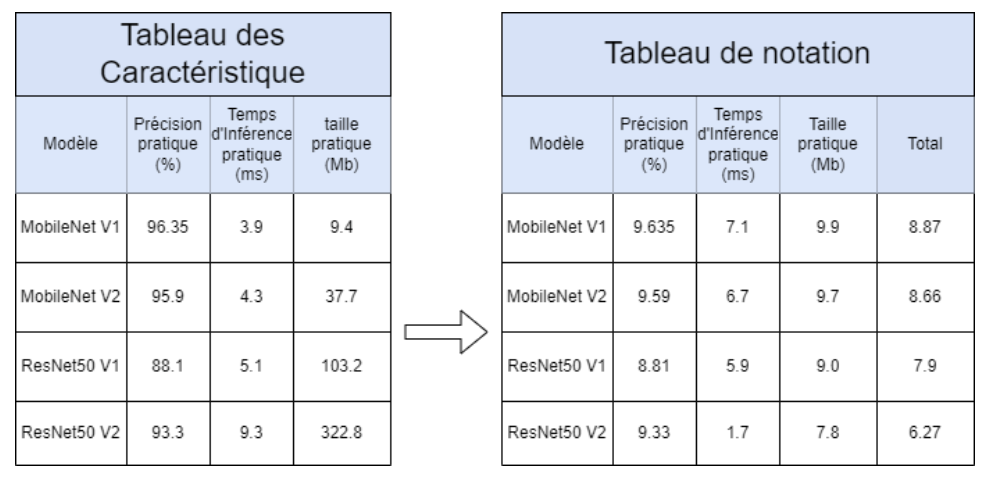
\includegraphics[width=13cm]{assets/PartTwo/ChapterTwo/TableauAnalyse.png}
    \caption{TableauAnalyse}
    \label{TableauAnalyse}
    \end{figure} 

    D'après la Figure \ref{TableauAnalyse}. Nous pouvons voir que les modèles MobileNet-V1 et MobileNet-V2 sont légèrement plus précis que le modèle Resnet50 V2. D'autre part, ResNet50-V1 est loin de cette comparaison car il a eu un effet d'overffiting qui montre une diminution de sa précision. Cela implique que l’hypothèse 1 est infirmée. 

    MobileNet-V1 est plus performant que les autres modèles en termes de temps d'inférence, car ses couches sont moins denses. Le MobileNet V2 est un peu proche au mobileNet V1 car il est aussi n’est pas dense en termes de couches convolutive. Le ResNet V1 et V2 malgré qu’ils ne soient pas dépasser les 10s mais ils ont toujours un peu lents par rapport de MobileNet V1. Donc l’hypothèse 2 est confirmée. 
    Les tailles des quatre modèles ont été modifiées car la méthode de transfert learning décrite précédemment dans le chapitre deux de la première partie implique l'ajout d'un nouveau classificateur (couches entièrement connectées) au modèle. 
    
    La taille augmentera donc proportionnellement à la taille du nouveau classificateur, mais même dans ce cas, la taille de MobileNet-V1 reste la plus petite par rapport aux autres modèles. Ceci implique que l'hypothèse 3 est infirmée car la taille du modèle à l'implémentation dépend du nouveau classificateur ajouté. 
    
    \newpage
    \section{Conclusion}
    Les trois hypothèses ont été traitées dans ce dernier chapitre par évalué chaque modèle selon les trois facteurs : la précision, le temps d'inférence et la taille du modèle. Grâce à l'application des modèles dans un cas réel. 

Ensuite, nous avons cité les hypothèses qui ont été réfutées et l'hypothèse unique qui a été confirmée. Enfin et après avoir considéré plusieurs itérations, nous avons finalement opté pour le modèle “MobileNet V1” en raison de ses performances d'implémentation. 

Ce modèle sera implémenté dans une solution complète de détection des nouilles non conforme. 

